\section{Validation}
\label{validation}

In order to quantify the value of this \textit{tranformational} approach, a validation tools is necessary. The extraction of Partially Observable Markov Decision Processes from Simulink model is simply a transformation between different dynamic system descriptions, a transformation from a rule based system description to a probabilistic state transitional system. Ideally such a transformation would produce a perfect representation of the source model. Unfortunately assumptions and simplifications (see sections~\ref{subsec:stateoutput}, \ref{subsec:outputdiscretization} and \ref{subsec:markovprop}) may have a derogatory effect on the quality of the system representation. The \textit{validator} aims to help identify the qualitative shortcomings of an extraction product. Using visual descriptive statistics tools such as box plots and simple correlation analysis, the validator provides a user of the extractor with means to verify the accuracy of the extracted dynamic system.

Chapter~\ref{results} presents an actual extraction result using the \textit{validator} to compare the respones of the original system and the extracted system.

% \subsection{Motivation}

% The motivation behind the development of a Markov Process validator is that

\subsection{Approach}

The \textit{validator} measures qualitative difference between two dynamic system descriptions by comparing the responses of the two systems to idential stimulation. The approach of analysing the response of a dynamic system to well-defined stimulation comes from the field of control, as this method can often provide insight into the system's behaviour. Linear time-invariant system are, for example, completely defined by their impulse response, ie. the reponse to other input signals can be deduced from the impulse response. Common stimulation signals include the Dirac Delta function, the Heaviside step function, sine functions or white noise.

This approach is based on the assumption that similar responses to identical stimulation implies similar system descriptions. Given that the \textit{extractor} simply transforms a model described in one way (Simulink) to a model described in another way (Markov Process) the response of these two systems should be similar given similar stimulation.

The difference between the responses of both systems may thus be an accurate measure of the qualitative deficit of the Markov Process description.

\subsection{MDP/POMDP Simulator}

In order to compare system reponses, the validator requires the ability to simulate Markov Processes. Given a fully defined MDP or POMDP and a decision array (containing an action for each decision epoch), a simulator must produce a response of the system as a historical series of states the process reached.

Therefore the validator includes an MDP simulator. Given an initial state and action set tuple the simulator samples as follows: at each epoch, a uniformly distributed number in the range $[0,1]$ is taken, the state the system will transition to in the next epoch is then chosen by comparing the uniform random number to the transition probability's cumulative distribution. This sequential sampling and transitioning loop continues until all actions have been taken and the historical state transitions is returned as the simulation output.

\subsection{Methodology}
\label{subsec:validationmethodology}

This section describes the methodology behind the validator. Because of the probabilistic nature of the systems studied in the context of Markov Processes, validation cannot rely on only individual simulations. In order to take into account the random differences between system responses, Monte Carlo simulations are required. Accurately comparing the responses of a Simulink model and an MDP model thus entails comparing response distributions instead of individual responses.

Box plots offer a way of representing distributions of values visually and are thus the validator's main output. A box plots takes a series of values and represents these values using a median mark, a box containing values between the 25th and 75th percentile, whiskers traditionally encompassing approximately 99.3\% of the data (if normally distributed) and finally individual outliers far of the norm.

Figure~\ref{boxplotexample} shows two example box plots, both produced with only one data series. The box plot on the left was produced using a range of only four values taken from the standard normal distribution and it is immediately obvious, that four values do not suffice for a clear representation of the normal distribution. Contrastingly, the box plot on the right was produced using one thousand random number taken from the same distribution. The law of large number dictates that the median should be nearly exactly zero and the variance symmetric; this is clearly the case here. This short example shows that box plots are a good tool for the visual representation of probabilistically distributed data.

The validator produces two sets of two box plots. Using a series of values for \textit{each} epoch, a box plot is created to show the distribution of those values at each epoch. Each set of box plots, shows distributions of results of Simulink simulations in the upper plot and distribution of results of the Markov Process simulation in the lower plot. The two sets differentiate in that the first produced set compares the system responses in the real number space, whilst the other set compares the system responses in the state space.

A simulink simulation produces values in the real number space, whilst a Markov Process simulation occurs in the state space. In order to compare these two results, the Markov Processes states must be mapped to real values, or the real values of the Simulink simulation must be mapped into the state space. The validator does both. After running multiple simulations of both the Simulink model and the Markov Decision Process, the validator converts the Simulink simulation output series to state transition series by searching the Markov Process's state space and finding the states that match the scalar values, and it converts the Markov Process simulation's state transition series into a series of real values simply by using the state definitions' rounded output value (see section~\ref{subsec:outputdiscretization}). The validator now has both the simulation result as an array of consecutive values as well as an array of consecutive states. Using both these descriptions, it produces box plots representing the distribution of both simulations' outputs and states.

Beside the box plot, the validator also produces a plot showing the correlation of the simulation result distributions in state space. It does this by calculating, for each epoch, the correlation between the state distribution vectors of the Simulink model's system response and the Markov Process's response.

Finally the validator also produces two plots using the mean output value (real numbers space) and the mean state-index (state space) of both the Simulink and the Markov Process simulations at each epoch. Although this plot provides valuable information, it must be considered carefully, as it no longer takes into account the variances of the responses, merely their means.

\begin{figure}
\begin{center}
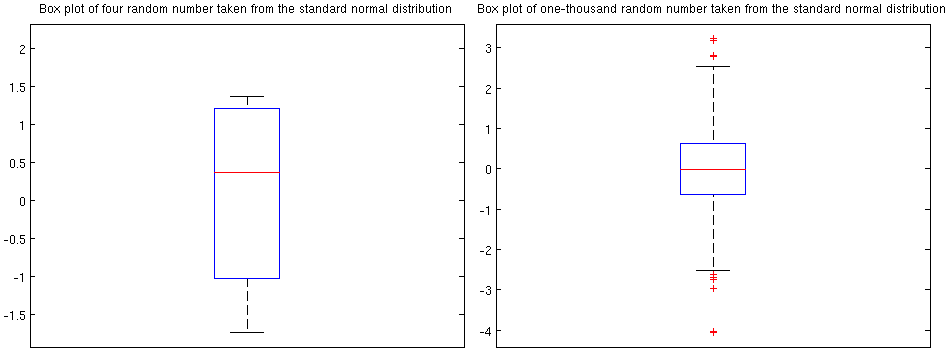
\includegraphics[width=16cm]{media/boxplotexample}\\
% 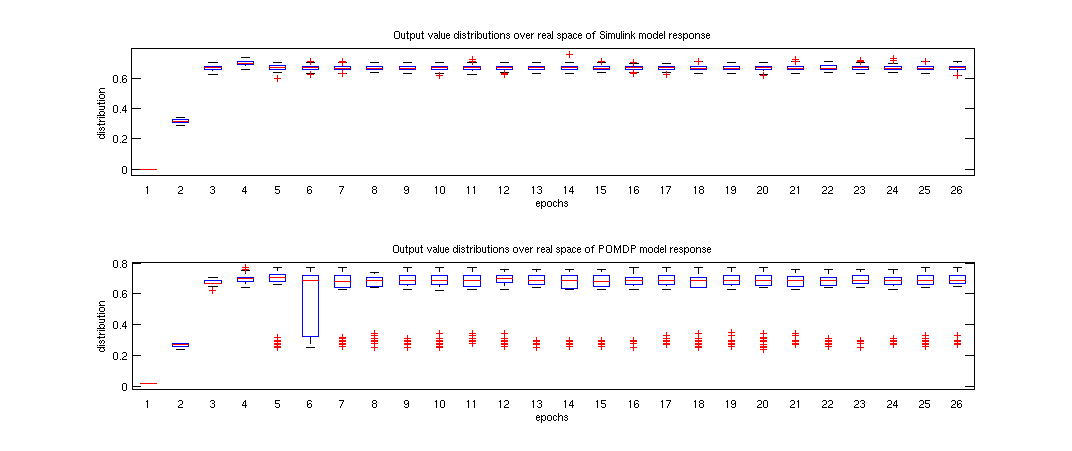
\includegraphics[trim 1cm 3cm 5cm 2cm, clip=true]{media/bw/bw_val_const_real_box}\\
\end{center}
\caption{Example box plots}
\label{boxplotexample}
\end{figure}


\subsection{Limitations}

This validation approach does have certain limitations. Mainly it is based on the assumption that similar responses imply similar system dynamics. Although this can be said of linear time-invariant systems, it may not be the case for other types of models. This must be kept in mind when assessing the quality of an extracted model. A number of other limitations exist.

Firstly the validator can only be used with single-output models. The response difference is not computed in the continuous domain, but rather in state space, meaning that the outputs of simulations of the Simulink models are mapped into the Markov Process's state space and then compared. In order to assess the variance of the two systems' responses, the state space must then be ordered. Unfortunately ordering only supports one-dimensional values (n-dimensional spaces cannot easily be ordered).

Additionaly a comparison of a continuous model with a discrete model requires the discretization of the former, meaning that the quality of the transformed model can only be judged as far as the discretization permits. Rough discretization parameters may hide some of the source model's underlying dynamics, yet still not be correctly recognized by this validation tool. The quality of its assessment is limited by the roughness of the transformation's discretization.

Finally the comparison is also limited by the conversion ratio between simulation time steps and Markov Process epochs (see section~\ref{subsec:timestepsdecisionepochs}). Because this ratio may be greater (but never less) than $1$, the dynamics of the system between epochs cannot be compared to the response of the Markov Process. This means that a comparison is only possible at every epoch, even though the original model may show significant non-linear behaviour between these time steps. The \texit{validator} can thus not provide a qualitative assessment of the differences between epochs.

% \subsection{Results}
% \label{subsec:validatorresults}

% The \textit{validator} produces a number of outputs that can be used to judge the quality of the transformation. Firstly it produces box plots of the distribution of the systems' response in state space over time. These plots can be used to assess the variance between the responses of the two systems. Secondly it produces a plot of the correlation between response distributions in state space for each time step, and finally it produces a plot of the mean of all simulation results of each system in real space over time.

% The \textit{validator} is a graphical validation tool that produces seven different plots that can be used to compare the responses of two dynamic systems. The following few paragraphs describe these plots and their meaning in more detail.

% The first output of a comparison is a box plot of the distribution 



% The \textit{Result} chapter uses the validation results to discuss the quality of the extraction of a Markov Process from a third-order Butterworth filter Simulink model.


% Using a traditional control systems approach, the tool compares the responses of both the original Simulink model and the produced Markov model to stimulation, stimulation being an artificially produced signal of input values. Figure~\ref{stepresponsefig} shows the response of a system to a commonly used stimulation, the Heavyside step function,

% \[
%   H[n] = \left\{ 
%   \begin{array}{l l}
%     0, & \quad n < 0\\
%     1 & \quad n \geq 0\\
%   \end{array} \right.
% \]

% Given a simulink model, an MDP or a POMDP and a stimulation signal, the validation tool runs hundreds of Simulink simulation and hundreds of MDP or POMDP simulation to produce the following:
% \begin{itemize}
% \item Box plot of the Simulink model state response (Simulink values are mapped to states within the MDP or POMDP's state space)
% \item Box plot of the MDP or POMDP state response
% \item Plot of the mean of the output value, for both the Simulink model and the MDP or POMDP, over time
% \item Plot of the correlation of the state distribution, of the Simulink model response and the MDP or POMDP response, at each time step
% \end{itemize}

% The \textit{validator} is however limited. In order to produce box plots over the state distributions it must order states. State can only be ordered if they are defined by only a single output value, thus limiting the \textit{validator} to single-output models.

% \begin{figure}
% \begin{center}
% 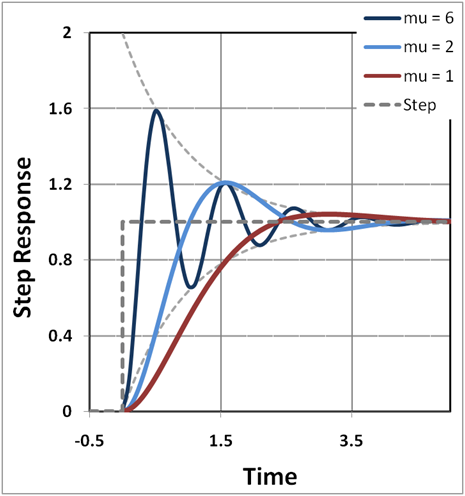
\includegraphics[height=8cm]{media/stepresponse_temp}\\
% \end{center}
% \caption{Step response of some system [XXX]}
% \label{stepresponsefig}
% \end{figure}
